\documentclass{article}

% if you need to pass options to natbib, use, e.g.:
%     \PassOptionsToPackage{numbers, compress}{natbib}
% before loading neurips_2018

% ready for submission
% \usepackage{neurips_2018}

% to compile a preprint version, e.g., for submission to arXiv, add add the
% [preprint] option:
%     \usepackage[preprint]{neurips_2018}

% to compile a camera-ready version, add the [final] option, e.g.:
     \usepackage[final]{neurips_2018}

% to avoid loading the natbib package, add option nonatbib:
%     \usepackage[nonatbib]{neurips_2018}

\usepackage[utf8]{inputenc} % allow utf-8 input
\usepackage[T1]{fontenc}    % use 8-bit T1 fonts
\usepackage{hyperref}       % hyperlinks
\usepackage{url}            % simple URL typesetting
\usepackage{booktabs}       % professional-quality tables
\usepackage{amsfonts}       % blackboard math symbols
\usepackage{nicefrac}       % compact symbols for 1/2, etc.
\usepackage{microtype}      % microtypography
\usepackage{graphicx}

\title{Hamiltonian Neural Networks}

% The \author macro works with any number of authors. There are two commands
% used to separate the names and addresses of multiple authors: \And and \AND.
%
% Using \And between authors leaves it to LaTeX to determine where to break the
% lines. Using \AND forces a line break at that point. So, if LaTeX puts 3 of 4
% authors names on the first line, and the last on the second line, try using
% \AND instead of \And before the third author name.

\author{%
  Ayush Garg \\
  Computer Science and Engineering\\
  Indian Institute of Technology Gandhinagar\\
  \texttt{ayush.g@iitgn.ac.in} \\
  % examples of more authors
   \And
   Sammed Shantinath Kagi \\
   Computer Science and Engineering \\
   Indian Institute of Technology Gandhinagar\\
   \texttt{sammed.shantinath@iitgn.ac.in} \\
  % \AND
  % Coauthor \\
  % Affiliation \\
  % Address \\
  % \texttt{email} \\
  % \And
  % Coauthor \\
  % Affiliation \\
  % Address \\
  % \texttt{email} \\
  % \And
  % Coauthor \\
  % Affiliation \\
  % Address \\
  % \texttt{email} \\
}


\begin{document}
% \nipsfinalcopy is no longer used

\maketitle

\begin{abstract}
In today's world, neural networks are being in almost every discipline resulting in significant improvement in all the tools and applications. But in the field of Physics, they struggle to attain the basic laws like conservation of momentum. The paper Hamiltonian Neural Networks addresses this issue by using Hamiltonian mechanics to train the neural network in an unsupervised method. The following report is an explanation of the paper and the code to reproduce the claimed results.
\end{abstract}

\section{Introduction}
Neural networks have the remarkable ability to learn and generalize underlying patterns in data. They have been known to give state-of-the-art results of most of the computational tasks. Due to this, much research goes into how to improve them in terms of accuracy, speeding their training time, and many other aspects. A relatively newer field where neural networks are applied is in Physics. Even today, neural networks given a task to predict the dynamics of a system are unable to learn the basic physical laws governing the whole system. Neural networks do not have any idea of the physical laws and learn them form the data instead. As the data is never perfect, learning only an approximation of the laws is possible. These laws behave close to the conservation laws underlying when observed for a short time frame, but in the long run, the cracks start to appear. Many researchers have tried to find these physical priors that transfer across tasks.

In this work, we reproduce the paper\footnote{Our code is available at github.com/ayushgarg31/HNN-Neurips2019} Hamiltonian Neural Network \cite{greydanus}. The approach presented in the paper takes inspiration from the Hamiltonian mechanics, a branch of physics that deals with conservation laws and invariances, and defines the concept of Hamiltonian Neural Networks (HNNs). The general idea of Hamiltonian mechanics is, to begin with, an equation called Hamiltonian, which relates various quantities of the system to a conserved quantity of the system and uses it to simulate how the system would ideally work. This equation is found using the domain-specific knowledge, but in the paper, the equation is learned by the Hamiltonian Neural Network on its own using the data.

As the official implementation \footnote{The official implementation is available at github.com/greydanus/hamiltonian-nn} of the experiments is already provided by the authors in pytorch\footnote{https://pytorch.org/}, we reproduce the results in Tensorflow. We reproduce their results for the ideal mass-spring system, ideal pendulum system, real pendulum system, 2-body system, 3-body system, pixel-pendulum system. We were able to reproduce their results for all the results, although their implementation for pixel pendulum didn't directly work for us and we came up with specific changes. We also experiment with a new system, real mass-spring system and provided our results and also point at some interesting insights from the data. In the rest of the sections, we will talk a little about the theory of Hamiltonian Neural Networks and then we will move on to our implementations and results.

\section{Theory}
\textbf{Predicting Dynamics}:\\
A Physics model is said to be complete if it can predict the changes in the system. As explained above, generic Neural Networks can follow the physical laws of conservation. This is the main goal, to learn the dynamics of a physics system in a Neural Network. So, to train the Neural Network, we make it predict the next state of the system from the current state. The past study on these concepts had a few theoretical problems with it as considering time to have discrete steps, not being able to follow the conservation laws. But as we know, time is continuous, so we define the model as a set of differential equations and integrate from the start time to close time. The following equation shows the calculation using the time derivatives of the states of the system (S)
\begin{equation}\label{sam0}
(q_1, p_1) = (q_0, p_0) + \int_{t_0}^{t_1} S(q,p) dt
\end{equation}
Since the neural networks are not able to conserve energy, the loss accumulates and affects later in the future. The HNN paper addresses the following 2 problems. To understand the concept of HNN we need to understand Hamiltonian Equations and Mechanics.\\
\noindent
\\
\textbf{Hamiltonian Mechanics:}\\
With a purpose to introduce classical mechanics in a more comprehensive unified manner, William Hamilton introduced the Hamiltonian Dynamics, which are now being used in every area of physics. \\
Using the data of positions $ q = (q_1, q_2, q_3, .....q_N) $ and the data of momentum's $ p = (p_1, p_2, p_3, .....p_N) $ we form N coordinated tuples which describes a complete system. Now we take a scalar function H(p,q) called Hamiltonian. So, the following equations give us the time evolution information of the system caused by the moving coordinates in the direction.


\begin{equation}\label{sam1}
\frac{dq}{dt} = \frac{dH}{dp}, \frac{dp}{dt} = \frac{dH}{dq}
\end{equation}
\begin{equation}
S_H = \left( \frac{dH}{dp}, - \frac{dH}{dq}  \right)
\end{equation}

This equation gives us the time evolution of the system. This gradient is a different type of gradient called "Symplectic Gradient." Moving a system in the direction of the gradients of H changes the output as quickly as possible, but moving in the direction of the Symplectic Gradient does no change the output. Using the above set of equations, we calculate the total energy of the systems in which energy is conserved. The importance of understanding Hamiltonian Mechanics is felt when working with systems with many degrees of freedom like celestial systems, fluid systems, etc.  




\section{Implementations and results}
In this section, we will talk about our implementations and results obtained using our implementations of the systems presented in the paper. All our implementations are in tensorflow\footnote{https://www.tensorflow.org/} v2.0.0-beta.

\textbf{Defining recurring expressions} - \(H\) is the conserved quantity (energy here), \(k\) is the spring constant, \(q\) is the position vector of the system, \(p\) is the momentum vector, \(m\) is the mass, \(g\) is the gravitational constant and \(l\) is the pendulum length. The state of the system is described using a concatenation of \((q, p)\).

\textbf{Details of neural networks -}\\
\textbf{Baseline - } It is a simple Multi-Layer Perceptron model which takes input the state of the system \((q, p)\), and outputs their time derivatives \((\partial q/\partial t, \partial p/\partial t)\). It has 3 dense layers, each with 200 hidden units with a \(tanh\) non-linearity function on the first 2 layers.

\textbf{Hamiltonian neural network - } In this architecture we input the state of the system \((q, p)\) and subject it to 3 dense layers each with 200 hidden units, out of which the last layer gives a scalar quantity which is the conserved quantity \(H\) neural network has learned. Then we differentiate the output of the 3 layers with respect to the input states and use the equation [\ref{sam1}] to get the time derivatives \((\partial q/\partial t, \partial p/\partial t)\). The differentiation is a part of the neural network itself.

\subsection{Ideal Mass-Spring system}
This was the first system we tried to reproduce results from the paper. First, we produce the data on which we will be training our HNN and test the results. To produce the data, we model the dynamics system of a friction-less mass-spring system using the Hamiltonian equation of the system.
\begin{equation}
H = \frac{1}{2}kq^2 + \frac{p^2}{2m}
\end{equation}
As in the paper, for simplicity we keep \(k = m = 1\). We make the dataset of trajectories of the ideal mass-spring system. For each trajectory, we randomly decide the total energy of the system uniformly distributed between [0.2, 1]. We use a differential equation to get the trajectory of the system and calculate differentials of state defining parameters \((q, p)\) with respect to time. Each trajectory has around 30 observations and we make a dataset of around 50 samples. We train the models on this dataset. After training, we use these models to predict \((\partial q/\partial t, \partial p/\partial t)\) given \((q, p)\), and use this to approximate the trajectory of the system using our differential equation given by equation [\ref{sam0}]. We then plot results of trajectories, MSE between coordinates, energy comparisons etc. to compare the learnings of the two models.\\
\textbf{Training details} - We used Adam optimizer \cite{kingma2014adam} with a learning rate of 0.001 to train the models. We trained models for 2000 iterations with a batch size equal to the size of the dataset. We use MSE loss to train our models.

\textbf{Results} - We were able to reproduce the results of claimed by the authors for this system.
\begin{figure}[htp]
    \centering
    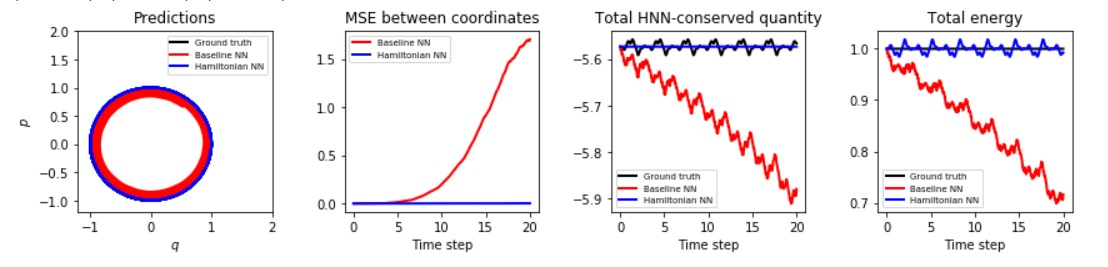
\includegraphics[width=15cm]{NeuRIPS2019/download.png}
    \caption{Analysis of models trained for ideal mass-spring system.}
    \label{fig:galaxy}
\end{figure}

The first plot is the trajectory followed by each of the models. As we can see, the baseline slowly drifts away from the ground truth, whereas the HNN follows ground truth with high accuracy, which is also evident from the second plot of coordinate comparisons. In the second graph, baseline coordinates diverge rapidly from ground truth, whereas for HNN it is almost perfect. Third and fourth graphs suggest that \(H\) learned by HNN resembles the total energy of the system and hence learns the conservation law pretty well, whereas the baseline does a terrible job at conserving the energy.

Measuring the energy MSE more quantitatively we get -\\
Baseline NN energy MSE: \quad 3.8732e-02 +/- 1.12e-02\\
Hamiltonian NN energy MSE: \quad 9.3688e-05 +/- 1.15e-05

\subsection{Ideal Pendulum system}
This was the second system we tried to reproduce results from the paper. First, we produce the data on which we will be training our HNN and test the results in a similar fashion as for the last system. The system is a little non-trivial one as, unlike the ideal mass-spring system, it is a non-linear dynamics system. The Hamiltonian equation of the system is given by.
\begin{equation}
H = 2mgl(1 - cos\:q) + \frac{l^2 p^2}{2m}
\end{equation}
Again we keep \(l = m = 1\). For each trajectory, we randomly decide the total energy of the system uniformly distributed between [1.3, 2.3] and \(g = 3\) as suggested in the paper. After, this all the steps remain the same as in the mass-spring system.\\
\textbf{Training details} - Training procedure and details remain the same as in ideal mass-spring system.

\textbf{Results} - We were able to reproduce the results of claimed by the authors for this system.
\begin{figure}[htp]
    \centering
    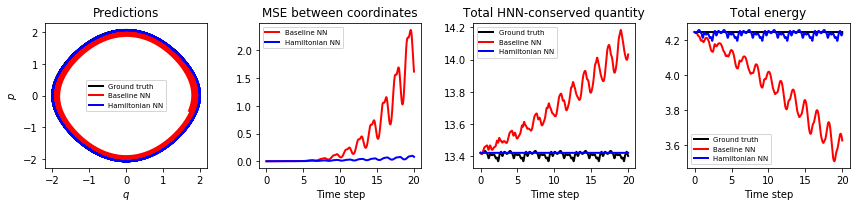
\includegraphics[width=15cm]{NeuRIPS2019/download1.png}
    \caption{Analysis of models trained for ideal pendulum system.}
    \label{fig:galaxy}
\end{figure}

Similar to the ideal mass-spring system, the first plot is the trajectory followed by each of the models. The baseline model slowly drifts away from the ground truth, whereas the HNN follows ground truth with high accuracy. In the second graph, baseline coordinates diverge rapidly from ground truth whereas for HNN it is almost perfect. Third and fourth graphs suggest that \(H\) learned by HNN resembles the total energy of the system, except it is negative in direction, same as in ideal mass-spring system.
Measuring the energy MSE more quantitatively we get -\\
Baseline NN energy MSE: 2.9537e-01 +/- 6.63e-02\\
Hamiltonian NN energy MSE: 3.6364e-02 +/- 6.77e-03

\subsection{Real Pendulum system}
This was the third system given in the paper. The data used in the task was from \textit{Science} paper by Schmidt & Lipson, which also tackled the problem of learning conservation laws from data. The data was much noisier and did not exactly follow any conservation law due to energy loss due to air resistance.

The training steps remain the same as in the ideal mass-spring system.\\
\textbf{Training details} - Training procedure and details remain the same as in ideal mass-spring system.

\textbf{Results} - We were able to reproduce the results claimed by the authors for this system.
\begin{figure}[htp]
    \centering
    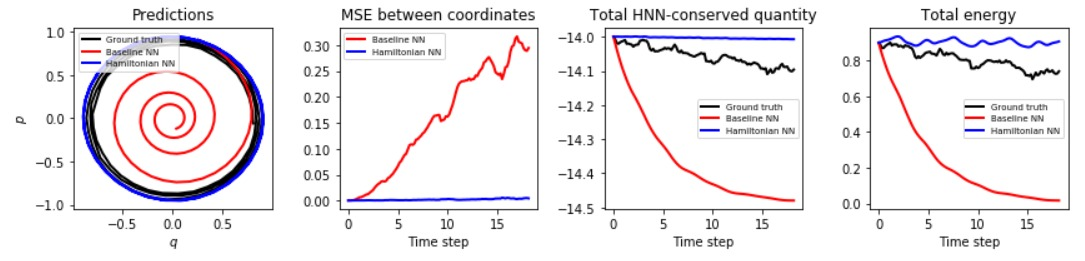
\includegraphics[width=15cm]{NeuRIPS2019/real-pendulum.png}
    \caption{Analysis of models trained for real pendulum system.}
    \label{fig:galaxy}
\end{figure}

In the first plot, we can see that the ground truth itself is not following conserved energy path but is rather collapsing very slowly. Although our HNN model cannot replicate this trajectory change due to energy loss but the loss is very slow, HNN gives a fine enough approximation. On the other hand baseline collapses too rapidly from its initial trajectory and hence does a very poor job at replicating the motion of a real pendulum. In the second graph, baseline coordinates diverge rapidly from ground truth, whereas for HNN it is still nearly perfect. Third and fourth graphs suggest that \(H\) learnt by HNN resembles total energy of the system and that the ground truth is losing some energy over time whereas baseline loses is pretty rapidly making a large drift between baseline and ground truth.

Measuring the energy MSE more quantitatively we get -\\
Baseline NN energy MSE: 3.4670e-01 +/- 7.20e-02\\
Hamiltonian NN energy MSE: 1.2575e-02 +/- 4.23e-03

\subsection{Two-body system}
This is a much more complex system compared to the ones presented till now as it involves the dynamics of two separate bodies in 2-dimension. In this system, the two bodies interact with each other due to a force such as gravitational force and influence each others' trajectory. The Hamiltonian for this system is given by.

\begin{equation}
H = \frac{|p_{CM}|^2}{m_1 + m_2} + \frac{|p_1|^2 + |p_2|^2}{2\mu} + g\frac{m_1m_2}{|q_1-q_2|^2}
\end{equation}

Here \(\mu\) is the reduced mass of the system, \(p_{CM}\) is the momentum of the center of mass of the system. In this system, each observation is of 8 dimensions, 2 for \(q\) of each body as it is 2 dimensional and similarly 2 for \(p\) of each body. For simplicity we keep \(m_1 = m_2 = g = 1\) and \(p_{CM}\) as zero as suggested in the paper.
For each trajectory, we start the system with the center of mass and total momentum as zero and distance between the two bodies randomly chosen uniformly chosen between [0.5, 1.5]. We add Gaussian noise to the trajectories with a variance of 0.05. We prepare a dataset of 200 trajectories with 50 observations each.

The training steps remain same as in the ideal mass-spring system.\\
\textbf{Training details} - Training procedure and details remain the same as in the ideal mass-spring system, although paper suggests to decrease the batch size and increase the gradient steps but our old procedure produces the same results as well.

\textbf{Results} - We were able to reproduce the results of claimed by the authors for this system.
\begin{figure}[htp]
    \centering
    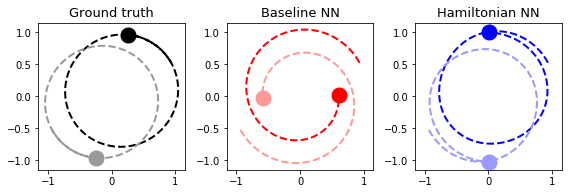
\includegraphics[width=10cm]{NeuRIPS2019/2_trajectory.png}
    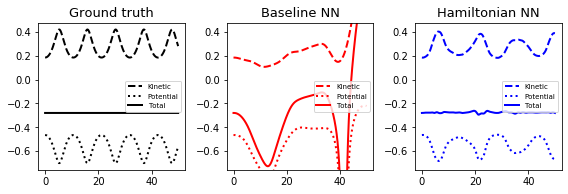
\includegraphics[width=10cm]{NeuRIPS2019/2_energy.png}
    \caption{Analysis of models trained for two-body system. First row shows the trajectories followed by each model and second row shows the potential, kinetic and total energies of each system.}
    \label{fig:galaxy}
\end{figure}

From the plots, we can see that HNN follows the trajectory of the two bodies and their energy trends quite accurately, whereas the baseline gives a completely unrecognizable plot of energies.

Measuring the energy MSE more quantitatively we get -\\
Baseline NN energy MSE: 1.3686e-01 +/- 5.59e-02\\
Hamiltonian NN energy MSE: 2.8087e-05 +/- 8.76e-06

\subsection{Three-body system}
In this experiment, two-body system is generalized to three bodies interacting with each other.
Most of the assumptions and hyper-parameters remain same as in two-body system.\\
\textbf{Training details} - Training procedure and details remain the same as two-body system.

\textbf{Results} - We were able to reproduce the results of claimed by the authors for this system.
\begin{figure}[htp]
    \centering
    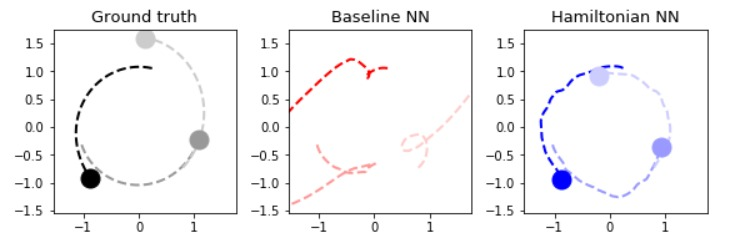
\includegraphics[width=10cm]{NeuRIPS2019/3_trajectory.png}
    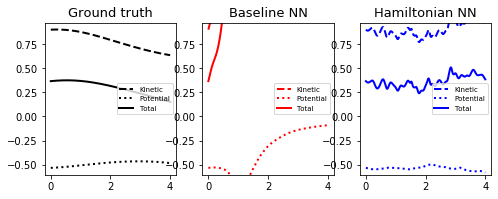
\includegraphics[width=10cm]{NeuRIPS2019/3_energy.png}
    \caption{Analysis of models trained for three-body system. First row shows the trajectories followed by each model and second row shows the potential, kinetic and total energies of each system.}
    \label{fig:galaxy}
\end{figure}

From the plots, we can see that although both the models do not have a very accurate replication of the ground truth but still HNN follows the trajectory of the two bodies and their energy trends somewhat satisfactorily whereas baseline gives a completely unrecognizable plot of energies and trajectories.

Measuring the energy MSE more quantitatively we get -\\
Baseline NN energy MSE: 5.4413e+07 +/- 1.44e+07\\
Hamiltonian NN energy MSE: 1.0903e+02 +/- 9.75e+01

\subsection{Pixel pendulum system}
Firstly we generate data using the OpenAI\footnote{https://gym.openai.com/} Gym's Pendulum-v0 environment. We generate 200 trajectories with 100 frames per trajectory, by down-sampling the original 400x400x3 images to 28x28x1 images. Then to get an estimate of velocity from the images, we concatenate 2 consecutive images together to make each data point of size 28x28x2. 

The task tackled in the paper is that given an image pair of 2 frames we need to output the next pair of frames. To use HNN and baseline model we first need to find a way to convert these pixel images to our known state variables \((q, p)\). To do this the paper uses an auto-encoder. Both the encoder and decoder of the auto-encoder were composed of four fully-connected layers with tanh activations and residual connections. There were 200 hidden units in each layer of both encoder and decoder and the output of encoder and input of decoder were of 2 units. The HNN and baseline models remain same. The idea was to encode the pixels to vector of size two and feed to our models and then decode the output of our models into pixel images again.

\textbf{Failures and modifications -} We encountered a number of problems while reproducing the results for pixel pendulum. We tried changing the smaller hyper-parameters like decreasing the learning rate, changed batch-size, increased number of iterations. After which we moved on to bigger changes, we changed the architecture a little, removed the residual part of the auto-encoder but we did not get the desired results.

After all these failures we turned to changing the training procedure. We tried to train auto-encoder separately and then use it as a separate entity to train HNN on it but it didn't work. Finally, we tried something very non-intuitive which actually worked. There are three types of losses used to train pixel HNN - auto-encoder loss is the loss in which given input, encode and decode it using auto-encoder and then take MSE, HNN loss is the loss in which it takes the input to encode it, run HNN on it and take MSE with the encoded next frames and the third one is the canonical coordinate loss which makes latent space look like (x, v) coordinates. In their implementation, they use a summation of all the three losses with HNN loss multiplied by 0.1. We found out that to train the models correctly, keep batch size 200 and do initial training for 25 epochs with learning rate \(10^{-3}\). Then start with only AE loss, start from a learning rate of \(10^{-3}\) and divide it by 10 every time fluctuation in losses start till learning rate gets to \(10^{-5}\), then add CC loss multiplied with 0.1 and train using similar pattern of learning rate, then increase multiplier to 0.5 and then later to 1. After this, add HNN loss with a multiplier of 0.1 and train in a similar fashion then change the multiplier to 0.5 and then finally to 1 at which stage do a final training for 25 epochs.

\textbf{Results} - We were able to reproduce the results of claimed by the authors for this system.
\begin{figure}[htp]
    \centering
    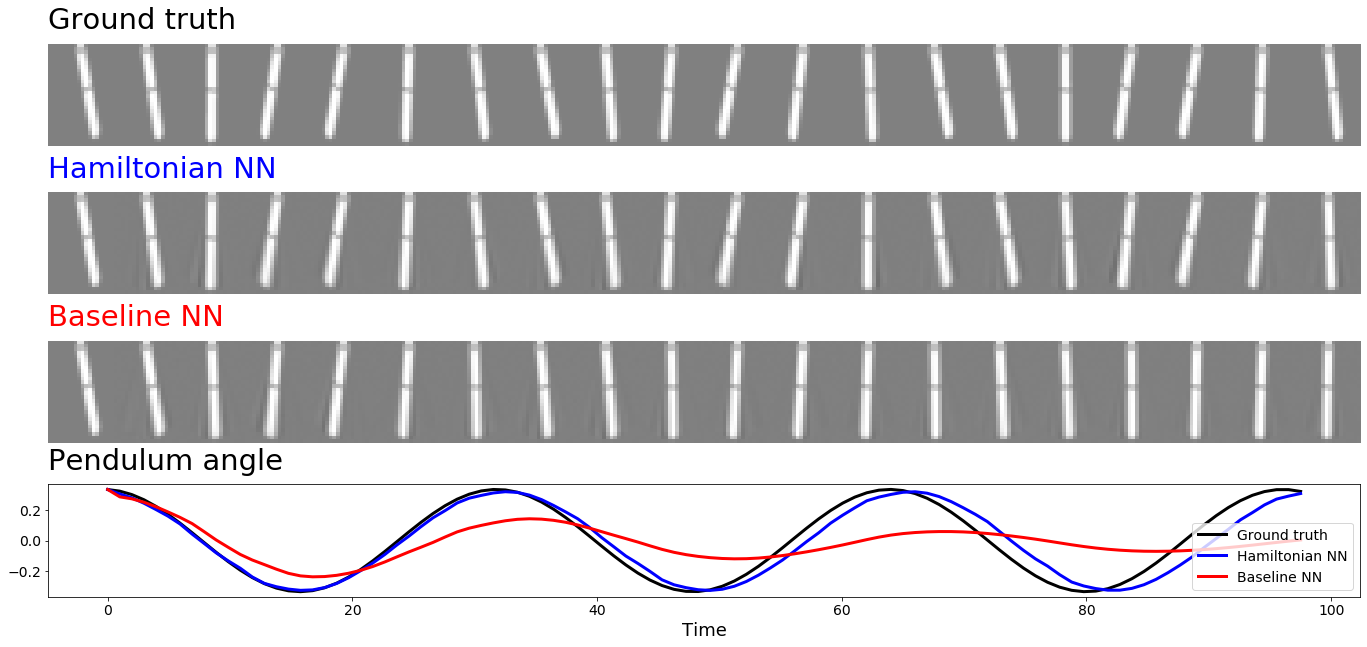
\includegraphics[width=10cm]{NeuRIPS2019/pixel.png}
    \caption{Analysis of models trained for pixel pendulum system.}
    \label{fig:galaxy}
\end{figure}

The plot shows how well the HNN models the ground truth while baseline starts losing energy and finally almost stops oscillating.

Measuring the energy MSE more quantitatively we get -\\
Baseline NN energy MSE: 1.6498e-01 +/- 4.78e-02\\
Hamiltonian NN energy MSE: 2.3617e-03 +/- 1.74e-04


\section{Real mass-spring system}
We planned to experiment with HNN on another real-world data and an obvious choice was real mass-spring system. We did an extensive search to find an available dataset that would be of use but unlike real pendulum system we couldn't find any. So, we modeled our own dataset with help from the Physics Department of our college. We have a mass-spring system similar to the ideal mass-spring system except that we also consider the damping effect of air resistance due to which slowly the system loses energy and motion of the system stops after a while. The force of air resistance is proportional to the velocity of the object. The force balance equation of the system is given by.

\begin{equation}
    ma + \beta v + kx = 0
\end{equation}
where \(a\) is acceleration of object, \(v\) is the velocity of the object, \(\beta\) is damping coefficient of air and \(x\) is the displacement from the position of equilibrium (where \(mg\) is balanced by spring force alone).

To prepare the dataset, till now we used the differential equations involving energy to predict the future state of the system. Here we cannot model the energy so easily as the energy is getting lost due to air resistance. Instead, we use a different method to predict the displacement, momentum and their time derivatives. It is similar to a Damped Harmonic Oscillator system. Hence we use the following equation to get the displacement of the object at any time.

\begin{equation}\label{sam7}
    x(t) = e^{\alpha t}(c_1 cos\:\omega t + c_2 sin\:\omega t)
\end{equation}
where \(\alpha = \frac{\beta}{2m}\), \(\omega = \frac{\sqrt{|\beta^2-4mk|}}{2m}\) and \(c1\) and \(c2\) are derived based on the initial conditions such as initial displacement and initial velocity of the object. Then this equation is differentiated to get velocity and momentum, which are then differentiated to get the time derivatives which are required to train our models.

For simplicity we keep \(k = m = 1\) and \(\beta\) is kept constant for each experiment. For each trajectory we randomly decide initial displacement from equilibrium position uniformly between [-5, 5]. We predict \((q, p)\) and \((\partial q/\partial t, \partial p/\partial t)\) for each observation using the differentials and double-differential of the equation [\ref{sam7}]. Each trajectory has around 200 observations and we make a dataset of around 50 samples. We further add Gaussian noise to the data with a variance of 0.1. The training procedure remains same as in ideal mass-spring system.\\
\textbf{Training details} - Training procedure and details remain the same as in ideal mass-spring system.

\textbf{Results} - We experimented on multiple values of \(\beta\) and found some interesting insights.

\begin{figure}[htp]
    \centering
    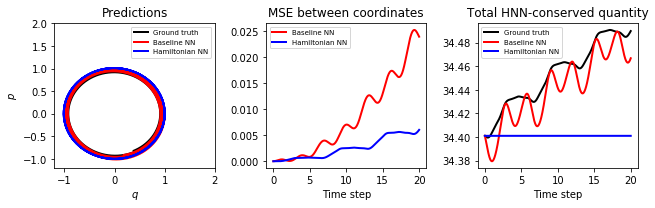
\includegraphics[width=12cm]{NeuRIPS2019/realmassspring.png}
    \caption{Analysis of models trained for real mass-spring system.}
    \label{fig:galaxy}
\end{figure}

The above plots are for \(\beta = 0.01\), the plots might be very interesting at first sight because although HNN performs better on coordinate prediction even though it is limited by constant energy constraint but surprisingly baseline does a much better work at replicating energy trends. We expect that the model which models energy better should also do better on coordinate prediction. We specifically chose to present plots with this \(\beta\), as this result is range specific.

Some interesting observations from experimenting the models with varying \(\beta\).
\begin{itemize}
  \item At very low values of \(\beta\), HNN performs better in both the tasks, of modelling coordinates and total energy as the system behaves much like an ideal mass-spring system where energy is almost conserved. At very high values \(\beta\), baseline performs  better in both the tasks as not only HNN is unable to replicate the loss in energy but also because baseline is very good at learning the pattern of loss.
  \item At the range close to 0.01 we see phenomenon similar to the one described above.
  \item Probably the most interesting of the observations is how accurately the baseline learns the pattern in energy loss. In the plot three (rightmost plot) we can not only see baseline and ground truth are close but also their periodicity is exactly the same (about 5 seconds) which is the same as the periodicity of the mass-spring system as well. Furthermore, in a single period, if we notice carefully the biggest dip in baseline comes when there is a dip in the ground truth and the smaller one comes along with a slight peak in the ground truth.
\end{itemize}

\section{Conclusion}
The results in the paper suggest that HNN is a solution to all the problems that are governed by physical laws. Although HNN is visibly better than a simple neural network when it comes to an ideal situation where energy is conserved but in real world, as we have seen in our experiment, most of the systems we know have an energy loss component and because of this, there is only a limited use of HNN, whereas baseline is much more general method and can even model real-world systems and also replicate energy loss with high precision which is not possible in HNN, especially when the loss is significant enough such that it cannot be ignored. Still the idea is pretty novel and can be built upon for further research. In addition to learning the conserved quantity, we can learn the trends in loss of the conserved quantity which can be much more useful tool for modeling real-world systems.

\bibliographystyle{plain} % We choose the "plain" reference style
\bibliography{NeuRIPS2019/refs}

\end{document}